\documentclass[11pt,pdftex,mathserif]{beamer}\usepackage[]{graphicx}\usepackage[]{color}
%% maxwidth is the original width if it is less than linewidth
%% otherwise use linewidth (to make sure the graphics do not exceed the margin)
\makeatletter
\def\maxwidth{ %
  \ifdim\Gin@nat@width>\linewidth
    \linewidth
  \else
    \Gin@nat@width
  \fi
}
\makeatother

\definecolor{fgcolor}{rgb}{0.345, 0.345, 0.345}
\newcommand{\hlnum}[1]{\textcolor[rgb]{0.686,0.059,0.569}{#1}}%
\newcommand{\hlstr}[1]{\textcolor[rgb]{0.192,0.494,0.8}{#1}}%
\newcommand{\hlcom}[1]{\textcolor[rgb]{0.678,0.584,0.686}{\textit{#1}}}%
\newcommand{\hlopt}[1]{\textcolor[rgb]{0,0,0}{#1}}%
\newcommand{\hlstd}[1]{\textcolor[rgb]{0.345,0.345,0.345}{#1}}%
\newcommand{\hlkwa}[1]{\textcolor[rgb]{0.161,0.373,0.58}{\textbf{#1}}}%
\newcommand{\hlkwb}[1]{\textcolor[rgb]{0.69,0.353,0.396}{#1}}%
\newcommand{\hlkwc}[1]{\textcolor[rgb]{0.333,0.667,0.333}{#1}}%
\newcommand{\hlkwd}[1]{\textcolor[rgb]{0.737,0.353,0.396}{\textbf{#1}}}%

\usepackage{framed}
\makeatletter
\newenvironment{kframe}{%
 \def\at@end@of@kframe{}%
 \ifinner\ifhmode%
  \def\at@end@of@kframe{\end{minipage}}%
  \begin{minipage}{\columnwidth}%
 \fi\fi%
 \def\FrameCommand##1{\hskip\@totalleftmargin \hskip-\fboxsep
 \colorbox{shadecolor}{##1}\hskip-\fboxsep
     % There is no \\@totalrightmargin, so:
     \hskip-\linewidth \hskip-\@totalleftmargin \hskip\columnwidth}%
 \MakeFramed {\advance\hsize-\width
   \@totalleftmargin\z@ \linewidth\hsize
   \@setminipage}}%
 {\par\unskip\endMakeFramed%
 \at@end@of@kframe}
\makeatother

\definecolor{shadecolor}{rgb}{.97, .97, .97}
\definecolor{messagecolor}{rgb}{0, 0, 0}
\definecolor{warningcolor}{rgb}{1, 0, 1}
\definecolor{errorcolor}{rgb}{1, 0, 0}
\newenvironment{knitrout}{}{} % an empty environment to be redefined in TeX

\usepackage{alltt}
% ewentualnie (w trakcie przygotowania prezentacji):
% \documentclass[...,handout]{beamer} % jedna 'frame' == jeden slajd
\usepackage[T1]{polski}        % jeśli po angielsku, to skasuj
\usepackage[polish]{babel}     % jeśli po angielsku, to skasuj
\selectlanguage{polish}        % jeśli po angielsku, to skasuj
\usepackage[T1]{fontenc}
\usepackage[utf8]{inputenc}  % kodowanie polskich znaków CP1250 (windows)
% Alternatywnie - latin2 dla kodowania ISO-8859-2 (raczej nie Windows)
% latex/pdflatex nie wspiera niestety Unicode (np. UTF-8)
\usepackage{amsmath,amssymb}     % więcej symboli matematycznych
\usepackage{graphicx}            % jeśli chcemy wstawiać grafikę
\usepackage{hyperref}            % odnośniki internetowe, zaawansowane ust. PDF
%\hypersetup{pdfstartview={FitW}}
\usepackage{natbib}
%%%%%%%%%%%% MOJE ULUBIONE USTAWIENIA BEAMERA %%%%%%%%%%%%%
%
\usetheme{Boadilla} % Warsaw to nazwa stylu - zmień na SWOJĄ ulubioną
\usecolortheme{spruce}
\useoutertheme{infolines}
\useinnertheme{circles}
\usefonttheme{structuresmallcapsserif}
%%
\setbeamertemplate{navigation symbols}{} % WYŁĄCZA PASEK NAWIGACJI U DOŁU
\setbeamercovered{invisible} % WPŁYWA NA WYŚWIETLANIE "SPAUZOWANYCH" ELEMENTÓW

%
\setbeamertemplate{theorems}[numbered]
\definecolor{green2}{rgb}{0.3, 0.6 ,0.4}
%
%%%%%%%%%%%%%%%%%%%%%%%%%%%%%%%%%%%%%%%%%%%%%%%%%%%%%%%%%%%
%
\title[Kategoryzacja tematyczna tekstów ]{Automatyczna kategoryzacja tematyczna tekstów przy użyciu metryk w przestrzeni ciągów znaków}
\author[N. Potocka]{Natalia Potocka}
%\institute[MiNI PW]{}
\date[11.10.2015]{11.10.2015}
%
%%%%%%%%%%%%%%%%%%%%%%%%%%%%%%%%%%%%%%%%%%%%%%%%%%%%%%%%%%%
%
\newtheorem{twierdzenie}{Twierdzenie}
\renewcommand{\proofname}{Dowód}
\newtheorem{lemat}[twierdzenie]{Lemat}
\newtheorem{wniosek}[twierdzenie]{Wniosek}
\newtheorem{stwierdzenie}[twierdzenie]{Stwierdzenie}

\theoremstyle{definition}
\newtheorem*{definicja}{Definicja}
\newtheorem*{oznaczenie}{Oznaczenie}

\newcommand{\R}{\mathbb{R}}
\newcommand{\N}{\mathbb{N}}
\newcommand{\E}{\mathbb{E}}
\newcommand{\xsr}{\overline{X}_n}
\newcommand{\skw}{S_n^2}
\newcommand{\al}{\alpha}
\newcommand*{\om}{\omega}


\newenvironment{zrodlo}{\emph{Źródło: }}{\par}
\IfFileExists{upquote.sty}{\usepackage{upquote}}{}
\begin{document}   % jedziemy :-)
%%%%%%%%%%%%% SLAJD TYTUŁOWY %%%%%%%%%%%%%%%%%%%%%%%%%%%%%%%%%%%%%%%%%%%%%
\thispagestyle{empty}% wyłącza paski na górze i na dole
\begin{frame}%

   \begin{center}%
%
%
%   %%%%%%%%%%%% NAGLOWEK %%%%%%%%%%%%%%%%%%%%%%%%%%%%%%%%%%%%%%%%%%%%%%%
%
      \begin{columns}%
         \begin{column}[c]{1.2cm}\centering%
         
\includegraphics[height=1.0cm]{logopw.pdf} \\%
         \end{column}

         \begin{column}[c]{7cm}\centering
            {\footnotesize{Politechnika Warszawska}}\\%
            {\footnotesize{Wydział Matematyki i~Nauk Informacyjnych}}%
         \end{column}

         \begin{column}[c]{1.2cm}\centering%
         
\includegraphics[height=1.0cm]{logomini.pdf} \\%
         \end{column}%
      \end{columns}

   %%%%%%%% TYTUL %%%%%%%%%%%%%%%%%%%%%%%%%%%%%%%%%%%%%%%%%%%%%%%%%%%%%%

      \vspace*{2em}

      \colorbox{green2}{\parbox{10cm}{\color{black}\centering\LARGE{Automatyczna kategoryzacja tematyczna tekstów przy użyciu metryk w~przestrzeni ciągów znaków}}}

      \vspace*{1.5em}%
      {\Large{Natalia Potocka}}\\%
%      {\color{blue}\footnotesize\texttt{M.Gagolewski@mini.pw.edu.pl}}

      %\vspace*{2.5em}%
      {\it\footnotesize Warszawa, 21.04.2014}  % DATA

   \end{center}

\end{frame}

%%%%%%%%%%%%%%%%%%%CZESC NATALII%%%%%%%%%%%%%%%%%%%%%%%%%%%%%%%%%%%%%%%%%%



\begin{frame}{Plan działania}
\begin{itemize}
  \item Cel pracy
  \item O metrykach słów kilka
  \item Postęp prac
  \item Co dalej?
\end{itemize}
\end{frame}


\begin{frame}{Cel pracy}
Celem pracy jest skategoryzowanie tekstów z~polskiej Wikipedii pod względem tematu na~podstawie liczności słów występujących w~tekście. Można się spodziewać, że~jeśli w~dwóch tekstach występuje dużo podobnych do~siebie słów, to~pochodzą one z~tej samej kategorii tematycznej. \\
\pause
\begin{tabular}{ |l r|l r|l r|l r| }
  \hline
  \multicolumn{2}{|c|}{A} & \multicolumn{2}{|c|}{B} & \multicolumn{2}{|c|}{C} & \multicolumn{2}{|c|}{D} \\
%  \multicolumn{8}{|c|c|c|c|}{A & B & C & D} \\
  \hline
  całka & 10 & całka & 5 & niewłaściwe & 3 & ułamek & 4 \\
  pochodna & 5 & pochodna & 15 & powieść & 7 & mianownik & 5 \\
  niewłaściwa & 4 & granica & 7 & granica & 15 & niewłaściwy & 6 \\
  \hline
\end{tabular}
\end{frame}


\begin{frame}{Cel pracy}
Co~ze~słowami podobnymi?\\
Przykładowo słowa \emph{niewłaściwy} i~\emph{niewłaściwa} mają ten sam temat, różnią się tylko rodzajem (męski / żeński). W tekstach mogą też występować błędy ortograficzne, błędy spowodowane brakami znaków diaktrycznych (\emph{ą, ę, ł, ...}) itd. Takie słowa również chcielibyśmy traktować jako ,,podobne''. W celu określenia jak bardzo dwa słowa są~do~siebie podobne, posłużą \emph{metryki określone na napisach}.
\end{frame}

% 
% \begin{frame}{O metrykach słów kilka}
% \begin{block}{Definicja}
% \emph{Napisem} nazywamy skończone złączenie symboli (znaków) ze~skończonego \emph{alfabetu}, oznaczonego przez $\Sigma$. Produkt kartezjański rzędu $q$, $\Sigma\times\ldots\times\Sigma$ oznaczamy przez $\Sigma^q$, natomiast zbiór wszystkich skończonych napisów, które można utworzyć ze~znaków z $\Sigma$ oznaczamy przez $\Sigma^*$. \emph{Pusty napis}, oznaczany $\varepsilon$, również należy do~$\Sigma^*$. Napisy zwyczajowo będziemy oznaczać przez $s$,~$t$~oraz $u$,~a~ich \emph{długość}, czyli liczbę znaków w napisie, przez $|s|$.
% \end{block}
% \pause
% Przykład. Niech $\Sigma$ będzie alfabetem złożonym z $26$ małych liter alfabetu łacińskiego oraz niech $s = 'ala'$. Wówczas mamy $|s| = 3$, $s \in \Sigma^3$ oraz $s \in \Sigma$. Pojedyncze znaki oznaczamy przez indeks dolny, stąd mamy $s_1 = 'a'$, $s_2 = 'l'$, $s_3 = 'a'$. %Podnapis oznaczamy przez $m:n$ w indeksie dolnym, np. $s_{1:2} = 'al'$. Jeśli $n < m$, to $s_{m:n} = \varepsilon$, czyli napis pusty.
% \cite{Loo2014:stringdist}
% \end{frame}
% 
% 
% \begin{frame}{O metrykach słów kilka}
% \begin{block}{Definicja}
% Funkcję $d$ nazywamy \emph{metryką} na~$\Sigma^*$, jeśli ma~poniższe własności:
% \begin{itemize}
% \item $d(s,t) \geq 0$
% \item $d(s,t) = 0$ wtw $s = t$
% \item $d(s,t) = d(t,s)$
% \item $d(s,u) \leq d(s,t) + d(t,u)$,
% \end{itemize}
% gdzie $s$,~$t$,~$u$~są~napisami.
% \end{block}
% \pause
% Nie wszystkie metryki na~napisach posiadają wszystkie z~wyżej wymienionych właśności.\\
% \pause
% Metryki na napisach można podzielić na~trzy grupy:
% \begin{itemize}
% \item oparte na~operacjach edytowania (\emph{edit operations})
% \item oparte na~$q$-gramach
% \item miary heurystyczne
% \end{itemize}
% \end{frame}
% 
% 
% \begin{frame}{O metrykach słów kilka}
% \begin{block}{Definicja}
% Funkcję $d$ nazywamy \emph{metryką} na~$\Sigma^*$, jeśli ma~poniższe własności:
% \begin{itemize}
% \item $d(s,t) \geq 0$
% \item $d(s,t) = 0$ wtw $s = t$
% \item $d(s,t) = d(t,s)$
% \item $d(s,u) \leq d(s,t) + d(t,u)$,
% \end{itemize}
% gdzie $s$,~$t$,~$u$~są~napisami.
% \end{block}
% Nie wszystkie metryki na~napisach posiadają wszystkie z~wyżej wymienionych właśności.\\
% Metryki na napisach można podzielić na~trzy grupy:
% \begin{itemize}
% \item \textbf{oparte na~operacjach edytowania} (\emph{edit operations})
% \item oparte na~$q$-gramach
% \item miary heurystyczne
% \end{itemize}
% \end{frame}
% 


\begin{frame}{Operacje edytowania}
Metryki oparte na operacjach edytowania zliczają liczbę opercji potrzebnych do~przetworzenia jednego napisu w~drugi. Najczęściej wymieniamymi operacjami~są:
\begin{itemize}
\item zamiana znaku, np. $'ala' \rightarrow 'ela'$
\item usunięcie znaku, np. $'ala' \rightarrow 'aa'$
\item wstawienie znaku, np. $'ala' \rightarrow 'alka'$
\item transpozycja dwóch przylegających znaków, np. $'ala' \rightarrow 'laa'$
\end{itemize}
\pause
Przykładowe metryki: Hamminga, najdłuższego wspólnego podnapisu (\emph{longest common substring}), Levenshteina, optymalnego dopasowania napisów (\emph{optimal string alignment}), Damareu-Levenshteina.

\end{frame}

\begin{frame}{Metryki oparte na operacjach edytowania}
Metryka \textbf{najdłuższego wspólnego podnapisu}, ozn. $d_{lcs}$, zlicza liczbę usunięć i~wstawień, potrzebnych do~przetworzenia jednego napisu w~drugi. Np. $d_{lsc}('leia', 'leela') = 3$, bo~$leela  \xrightarrow{us.\ e} lela  \xrightarrow{us.\ l} lea  \xrightarrow{wst.\ i} leia$.\\
\pause
\textbf{Odległość Levenshteina}, ozn. $d_{lv}$ zlicza sumę usunięć, wstawień oraz zamian znaków, potrzebnych do~przetworzenia jednego napisu w~drugi. \\


\pause
np.
$d_{lv}('leia', 'leela') = 2$, bo $leela  \xrightarrow{us.\ e} lela  \xrightarrow{zm.\ l\ na\ i} leia$. 
\end{frame}



\begin{frame}{Metryki oparte na operacjach edytowania}
Metryka \textbf{optymalnego dopasowania napisów}, ozn. $d_{osa}$, zlicza liczbę usunięć, wstawień, zamian oraz transpozycji przylegających znaków, potrzebnych do~przetworzenia jednego napisu w~drugi. Np. $d_{osa}('leia', 'leela') = 2$, bo $leela  \xrightarrow{us.\ e} lela  \xrightarrow{zm.\ l\ na\ i} leia$. \\
\end{frame}

\begin{frame}{Postępy prac}
Co zostało zrobione?\\
\begin{itemize}
\item wczytano $1\ 075 \ 568$ artykułów z polskiej Wikipedii \pause
\item razem to $2\ 806\ 765$ różnych słów... \pause
\item ... z czego $49\%$ wystąpiło tylko w \textbf{jednym} tekście
\item ... a $44\%$ wystąpiło tylko \textbf{jeden raz} we~wszystkich tekstach
\end{itemize}
\pause
Po usunięciu tzw. \emph{stopwords}, czyli słów nieistotnych w~kontekście analizy, jak np. \emph{a, bo, co, jak, to, w, z, że}, słów jednoliterowych oraz słów w~językach obcych z~niełacińskiego alfabetu, pozostało $2\ 805\ 858$ słów do~analizy.\\
\end{frame}



\begin{frame}{Postępy prac}
\begin{figure}[h]
      \centering
      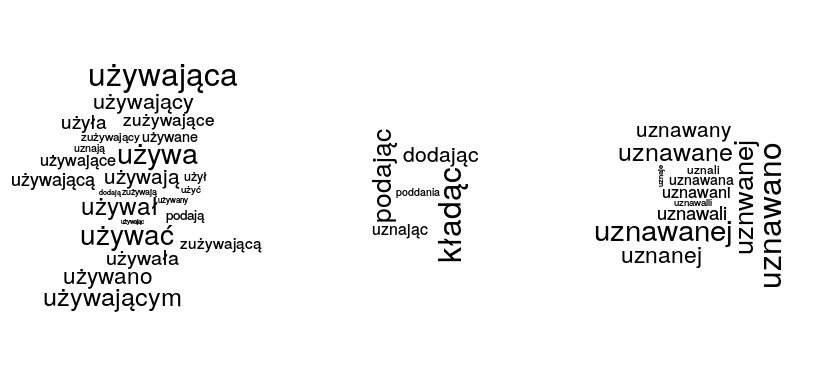
\includegraphics[width=12cm] {lv}
      \caption{Przykładowe grupy utworzone przy pomocy metryki Levenshteina. Maksymalna odległość w~klastrze to~$7$.}
    \end{figure}
\end{frame}



\begin{frame}{Postępy prac}
\begin{figure}[h]
      \centering
      
\includegraphics[width=12cm] {lcs}
      \caption{Przykładowe grupy utworzone przy pomocy metryki $lcs$. Maksymalna odległość w~klastrze to~$7$.}
    \end{figure}
\end{frame}



\begin{frame}{Postępy prac}
\begin{figure}[h]
      \centering
      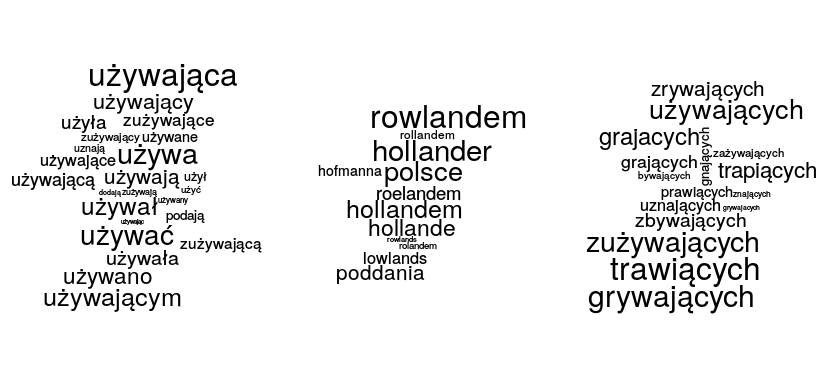
\includegraphics[width=12cm] {osa}
      \caption{Przykładowe grupy utworzone przy pomocy metryki $osa$. Maksymalna odległość w~klastrze to~$7$.}
    \end{figure}
\end{frame}



\begin{frame}{Postępy prac}
Z~powodu słabej jakości grupowania oraz braku możliwości obliczeniowych dokonano grupowania przy pomocy tzw. \emph{stemmingu}. Polega on~na~przyporządkowaniu do~słowa jego rdzenia, a~więc takiej jego części, która jest odporna na odmiany przez rodzaje, przyimki, przypadki itd.\\
Przykładowo dla słowa \emph{używająca} rdzeniem jest \emph{żyw}.\\
\pause
Do~stemmingu użyto narzędzia Hunspell, które sprawdza pisownię dla wielu programów, takich jak:  OpenOffice, Mozilla Firefox, Thunderbird czy Google Chrome.\\
Dzięki niemu udało się poklastrować $733\ 828$ słów ($\approx 26\%$ wszystkich) z~czego $89\%$ stanowiły polskie słowa $5,5\%$ - słowa angielskie, a~po~ponad $2\%$ - słowa francuskie i niemieckie. Innych języków nie sprawdzano. Liczba uzyskanów grup (klastrów) to~$186\ 942$.\\
\end{frame}

\begin{frame}{Postępy prac}
Co z pozostałymi słowami?\\
Słowa, które wystąpiły więcej niż raz we~wszystkich tekstach, dołączono do~już istniejących grup przy pomocy metryk. Takich słów było $973\ 855$, co~dało łącznie pogrupowanych słów w~liczbie $1\ 707\ 683$. Co więcej, grupy, które miało mało słów (między $1$ a $5$) połączono lub dołączono do innych zbiorów. W ten sposób uzyskano 13 różnych zbiorów grup słów.
\end{frame}


\begin{frame}{Postępy prac}
\begin{figure}[h]
      \centering
      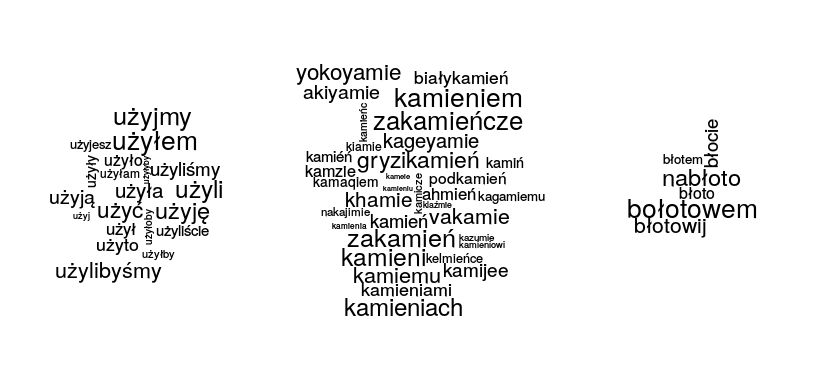
\includegraphics[width=12cm] {clust_all2}
      \caption{Przykładowe klastry utworzone przy pomocy Hunspella oraz metryki $lcs$.}
    \end{figure}
\end{frame}


\begin{frame}{Postępy prac}
Następnie dla próbki tekstów z~trzech kategorii: matematyka, historia sztuki oraz wojny, dokonano grupowania artykułów. Kryterium była liczność \textbf{grup słów} występujących w~danym tekście. Do grupowania użyto metody \emph{sferycznych $k$-średnich}.
% \pause
% \begin{block}{Przypomnienie}
% W~metodzie $k$-średnich minimalizujemy
% $$
% \sum_i d(x_i, p_{c(i)}),
% $$
% gdzie $x_i$ to~zbiór wektorów cech, $c(i) \in \{1,\ldots,k\}$ to~indentyfikator klastra, $p_1,\ldots,p_k$ to~środek klastra, a~$d$~to~odległość euklidesowa.
% \end{block}
\end{frame}

% \begin{frame}{Postępy prac}
% W~metodzie $k$-średnich minimalizujemy
% $$
% \sum_i d(x_i, p_{c(i)}),
% $$
% gdzie $x_i$ to~zbiór wektorów cech, $c(i) \in \{1,\ldots,k\}$ to~indentyfikator klastra, $p_1,\ldots,p_k$ to~środek klastra, a~$d$~to~odległość euklidesowa.
% \begin{block}{Metoda sferyczna}
% W~metodzie sferycznych $k$-średnich minimalizujemy \cite{Hornik2012:sphkmeans, Wild2002:sphkmeans}
% $$
% \sum_i d(x_i, p_{c(i)}) = \sum_i 1-\cos(x_i, p_{c(i)}) = \sum_i 1-\frac{<x_i, p_{c(i)}>}{||x_i||\cdot ||p_{c(i)}||},
% $$
% \end{block}
% \end{frame}

% 
% \begin{frame}{Postępy prac}
% W metodzie $k$-średnich minimalizujemy
% $$
% \sum_i d(x_i, p_{c(i)}),
% $$
% gdzie $x_i$ to zbiór wektorów cech, $c(i) \in \{1,\ldots,k\}$ to indentyfikator klastra, $p_1,\ldots,p_k$ to środek klastra, a $d$ to odległość euklidesowa.
% \begin{block}{Metoda sferyczna}
% W metodzie sferycznych $k$-średnich minimalizujemy
% $$
% \sum_i d(x_i, p_{c(i)}) = \sum_i 1-\cos(x_i, p_{c(i)}) = \sum_i 1-\frac{<x_i, p_{c(i)}>}{||x_i||\cdot ||p_{c(i)}||},
% $$
% \end{block}
% \end{frame}


\begin{frame}{Postępy prac}
Opierając się na~kategoriach z~Wikipedii, poprawnie sklasyfikowanych zostało $61\%$ z $59\ 403$ artykułów.
\begin{tabular}{|l|l|r|r|}
  \hline
tytuł & kat & id\_kat & kl \\ 
  \hline
kościół św. rocha w poznaniu & szt & 1 & 1 \\ 
  portret & szt & 1 & 2 \\ 
  quantum of solace (gra komputerowa) & szt & 1 & 2 \\ 
  kurka wodna (seria gier) & szt & 1 & 2 \\ 
  technika macierzy rzadkich & mat & 2 & 2 \\ 
  kryterium walda & mat & 2 & 2 \\ 
  generalized markup language & mat & 2 & 2 \\ 
  czesław falkiewicz & woj & 3 & 3 \\ 
  william goodenough & woj & 3 & 3 \\ 
  kazimierz gallas & woj & 3 & 3 \\ 
  wacław krzywiec & woj & 3 & 3 \\ 
  fabian aleksandrowicz & woj & 3 & 3 \\ 
   \hline
\end{tabular}

% 
% <<echo=FALSE>>=
% library(xtable)
% outcome2 <- readRDS("/home/natalia/Text-clustering-basing-on-string-metrics/Seminarium/art_clust_res2.rds")
% rzedy <- sample(1:nrow(outcome2), 12)
% tab <- outcome2[rzedy, c('title', 'kat_id','kat_id2', 'cluster')]
% tab <- tab[order(tab$kat_id2),]
% names(tab) <- c("tytuł", "kat", "id_kat", "kl")
% tab_out <- xtable(tab)
% digits(tab_out) <- 0
% align(tab_out) <- "|r|l|l|r|r|"
% print((tab_out),include.rownames=FALSE,floating=FALSE)
% @
% 
\end{frame}


\begin{frame}{Postępy prac}
Metoda ta dała dość dobre rezultaty dla małej próbki i małej liczby tematów. Dla większej liczby tematów i większej próbki, R miał problemy z pamięcią... \\ \pause
Stąd pomysł użycia metody mini-batch kmeans w pythonie. Dla $20\ 482$ artykułów i $981$ tematów, obliczenia  trwały ok. 70s. Wyniki dokładności były trochę gorsze, tzn. ok. $59\%$ artykułów z tego samego tematu znalazło się w tej samej grupie.\\ \pause
\begin{figure}[h]
      \centering
      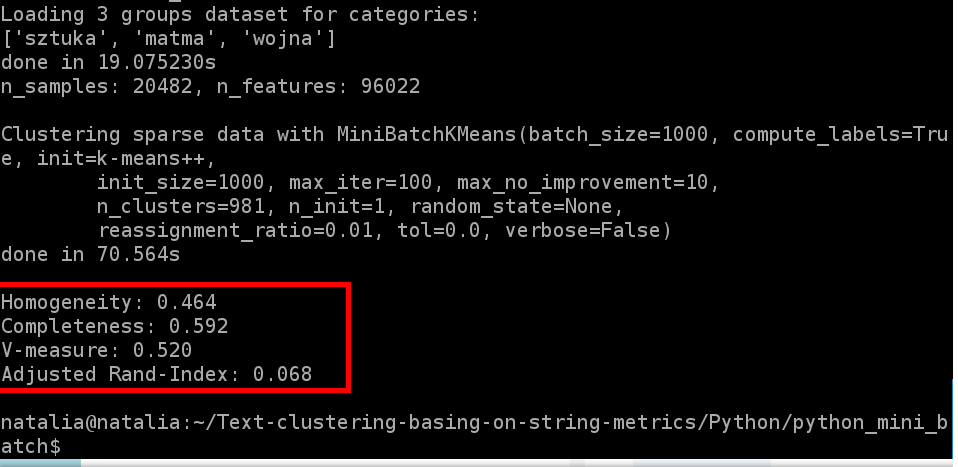
\includegraphics[width=10cm] {mini_batch_981_clusters.png}
      \caption{Czas i wyniki dla mini-batch kmeans.}
    \end{figure}
\end{frame}



\begin{frame}{Postępy prac}
Postanowiono puścić obliczenia na jednym ze zbiorów na wszystkich artykułach ($1\ 075\ 464$), dla $67\ 969$ tematów. Same dane wczytywały się $3$ godziny i zajęły... \pause $100$ GB RAMu (+swap). I algorytm liczył... i liczył... \pause Po 22 dniach stwierdziłam, że czas przerwać obliczenia.\\ \pasue
\begin{figure}[h]
      \centering
      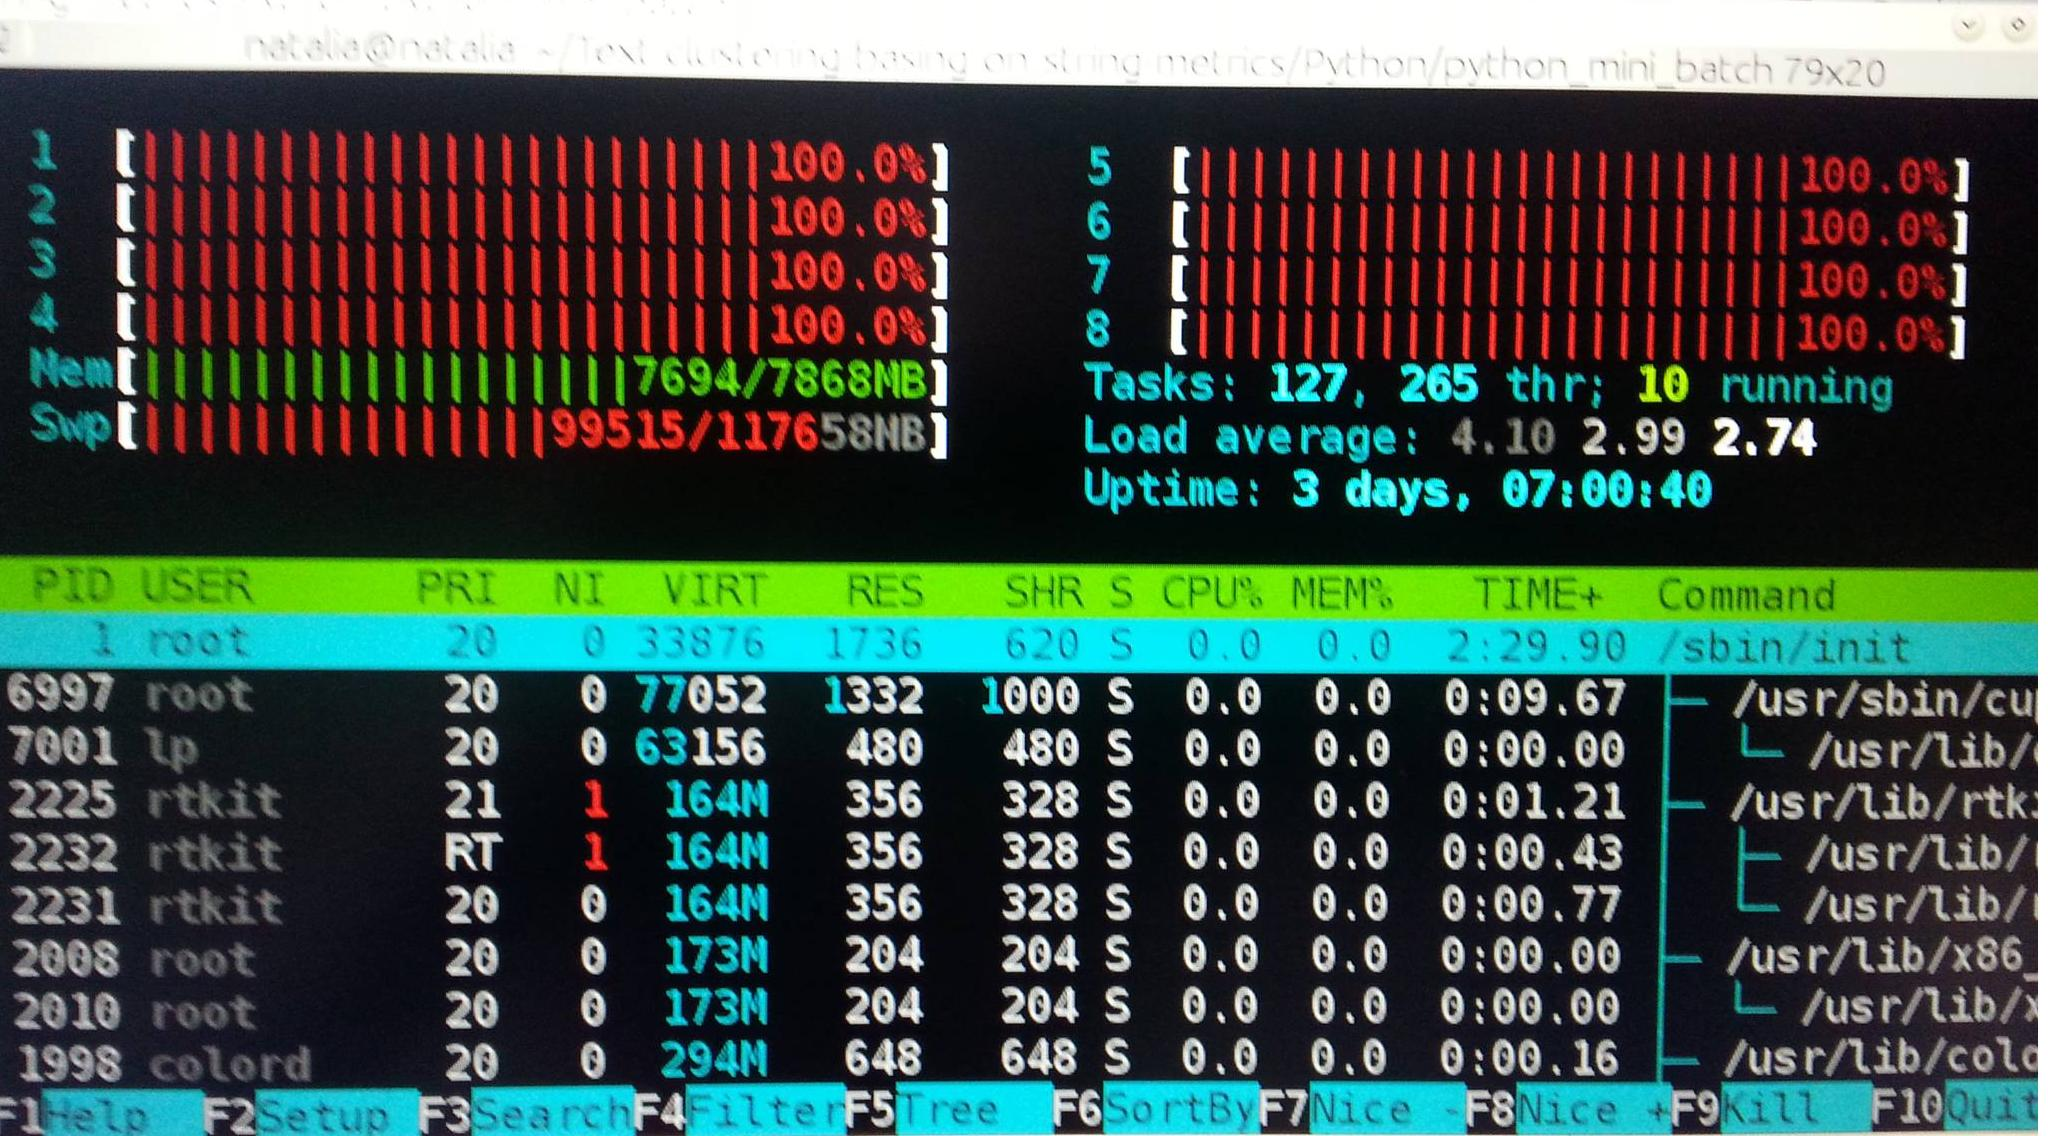
\includegraphics[width=10cm] {obl1.jpg}
      \caption{Czas i zużycie dla mini-batch kmeans.}
    \end{figure}
\end{frame}
 

\begin{frame}{Postępy prac}
Kolejne testy wykazały, że bardzo duża liczba tematów powoduje, że obliczenia przetwarzają się w nieskończoność. W tej chwili jestem na etapie zmniejszenia liczby tematów i rozproszenia obliczeń na kilka(-naście) komputerów.
\end{frame}


\begin{frame}{Bibliografia}
\nocite{Hornik2012:sphkmeans}
\nocite{Wild2002:sphkmeans}
\nocite{Loo2014:stringdist}
\bibliographystyle{plain}
\bibliography{bibliography}
\end{frame}


% \begin{frame}{Bibliografia}
% 
% \begin{thebibliography}{}
% \bibitem[1]{AS} Ananda Sen, \textit{On the Interrelation Between the Sample Mean and Sample Variance}, The American Statistician, 66 (2012), 112-117.
% %\bibitem[2]{CZ} L. N. de Castro, F. J. Von Zuben, "\href{http://www.dca.fee.unicamp.br/~vonzuben/research/lnunes_dout/artigos/gecco00.pdf}{\textit{The Clonal Selection Algorithm with Engineering Applications}}", GECCO 2000, Workshop on
% %        Artificial Immune Systems and Their Applications, Las Vegas, USA, str.
% %        36-37, 2000.
% %\bibitem[3]{M} \href{http://mst.mimuw.edu.pl/lecture.php?lecture=mbm&part=Ch12}{http://mst.mimuw.edu.pl/lecture.php?lecture=mbm&part=Ch12}
% %\bibitem[4]{IPIPAN} \href{www.ipipan.waw.pl/\~{}stw/ais/daaisy.html}{www.ipipan.waw.pl/\~{}stw/ais/daaisy.html}
% 
% 
% 
% \end{thebibliography}
% \end{frame}

\begin{frame}{}
   \begin{center}
      \Huge{Dziękuję za uwagę.}
   \end{center}
\end{frame}



\end{document}
